\documentclass[10pt]{beamer}

%\usetheme{Montpellier}
\usetheme{Madrid}

\usecolortheme{beaver}
\usepackage{appendixnumberbeamer}
\usepackage[utf8]{inputenc}
\usepackage[spanish]{babel}
\usepackage{booktabs}
\usepackage[scale=2]{ccicons}
\usepackage{pgfplots}
\usepgfplotslibrary{dateplot}
\usepackage{xspace}
\usepackage{csquotes}
\usepackage{graphicx}
\usepackage{verbatim}
\usepackage{listings}

\newcommand{\themename}{\textbf{\textsc{metropolis}}\xspace}
\graphicspath{ {images/} }

\title{Proyecto final de Procesamiento de Lenguaje Natural 2017}

\subtitle{Entrenamiento y validación de \textit{Fasttext} para el Castellano}

\date{Septiembre de 2017}

\author{Juan M. Scavuzzo}

\begin{document}

\maketitle



\begin{frame}{Fasttext}
  \begin{itemize}[<+->]
    \item Librería de Facebook AI Research % \cite{Fasttext}
    \item Open Source
    \item Diseñada para representación y clasificación de texto
      \begin{itemize}[<+->]
        \item Word Embeddings (skipgram, cbow)
        \item Clasificación supervisada
      \end{itemize}
   \item Ya hay entrenados modelos de embeddings para muchos idiomas
  \end{itemize}
\end{frame}


\begin{frame}{Problema}
    \begin{itemize}[<+->]
      \item Evaluar el performance de un modelo entrenado con un GRAN corpus
      \item Param tunning básico
      \item Generar embeddings orientados a sintaxis
    \end{itemize}
\end{frame}


\begin{frame}{Modelo: Entrenamiento - Corpus}
  Spanish Billion Word Corpus (~ 10GB)
  \begin{itemize}[<+->]
    \item Se usó el corpus que recopiló Cristian
    \item Se dejó de lado: php, ubuntu, openoffice3 y kde
  \end{itemize}
\end{frame}


\begin{frame}{Modelo: Entrenamiento - Preprocesamiento}
  \begin{itemize}[<+->]
      \item Se quitaron todos los simbolos no alfanuméricos
      \item Se generaron tokens de:
        \begin{itemize}[<+->]
          \item Números correspondientes a fechas
          \item Flotantes
          \item Enteros
          \item Abreviaciones (muy mejorable)
        \end{itemize}
      \item No se tocaron las stop-words
  \end{itemize}

\end{frame}


\begin{frame}{Modelo: Entrenamiento - Param Tunning}
  \begin{itemize}
    \item Dimensión de los vectores (100 - 300)
    \item Tamaño del n-gram (1 - 3)
  \end{itemize}
  \begin{center}
    A mano
  \end{center}
\end{frame}


\begin{frame}{Modelo: Validación - Word2Vec}
  \begin{center}
    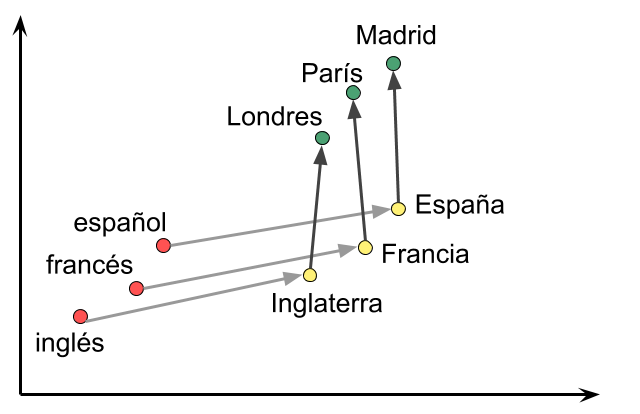
\includegraphics[width=0.8\textwidth]{word_vec.png}
  \end{center}
\end{frame}

\begin{frame}{Modelo: Validación - Word2Vec accuracy}

  \begin{center}
    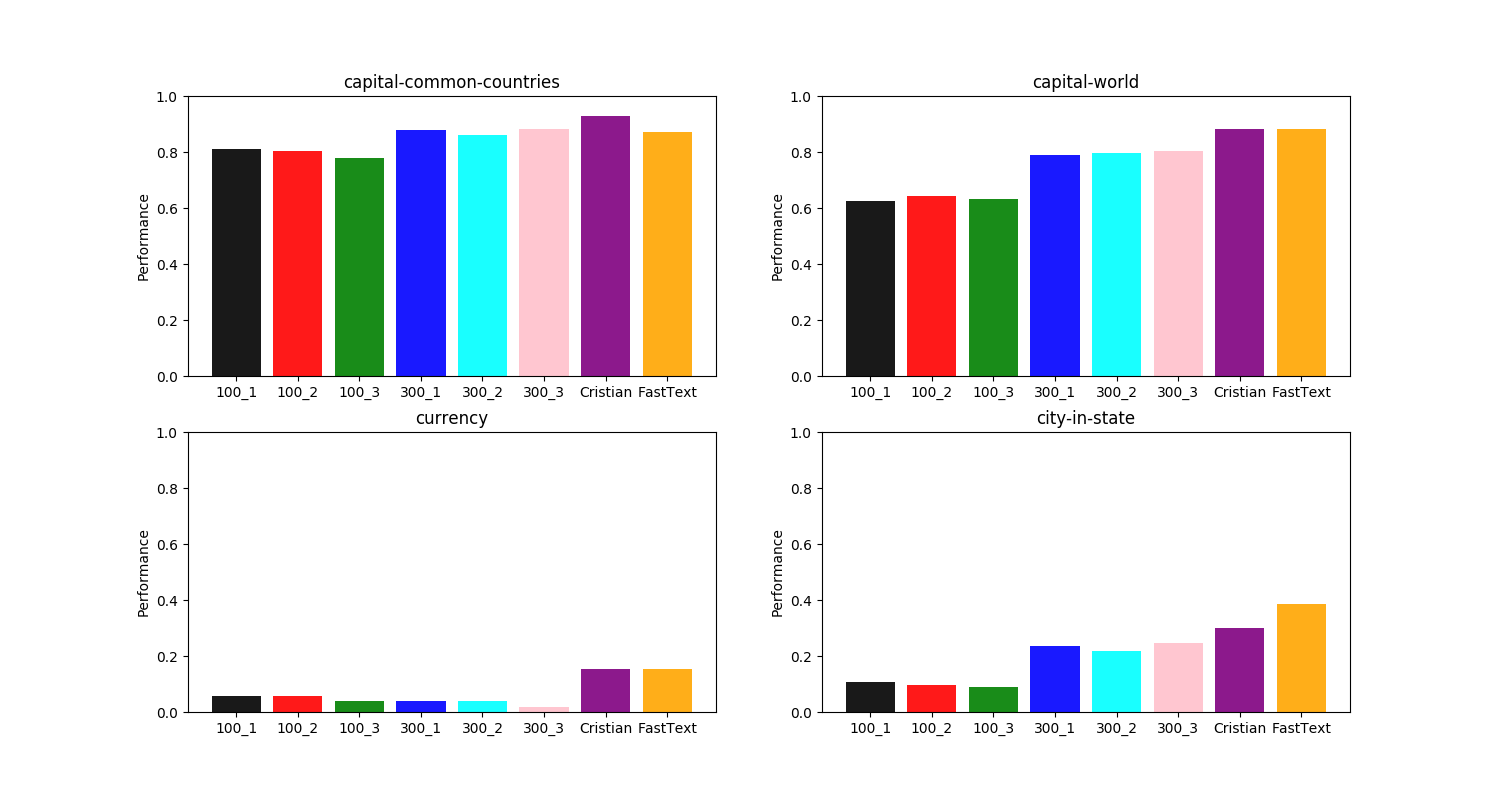
\includegraphics[width=1\textwidth]{plot1.png}
  \end{center}

\end{frame}


\begin{frame}{Modelo: Validación - Word2Vec accuracy}
  \begin{center}
    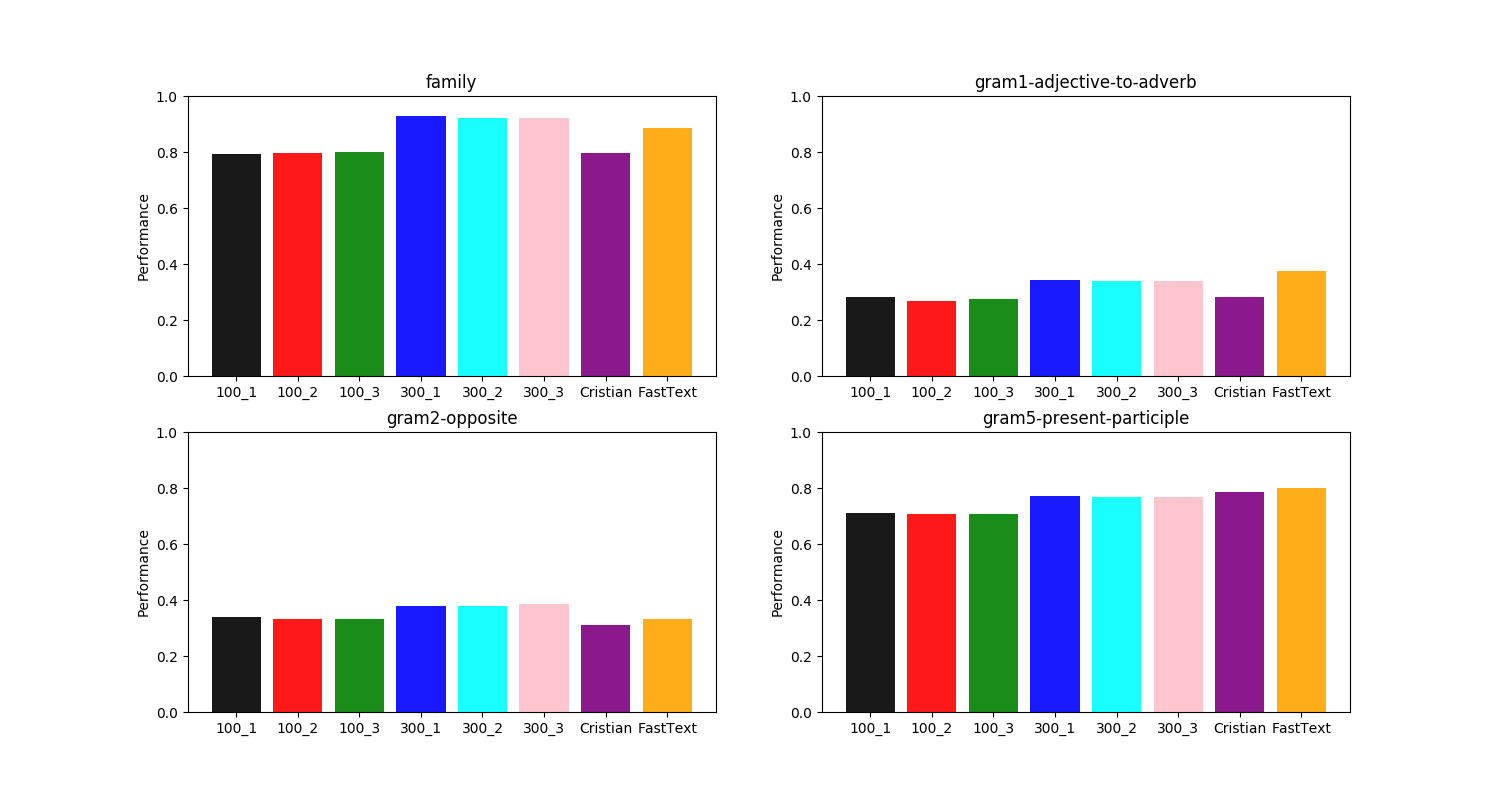
\includegraphics[width=1\textwidth]{plot2.png}
  \end{center}
\end{frame}

\begin{frame}{Modelo: Validación - Word2Vec accuracy}
  \begin{center}
    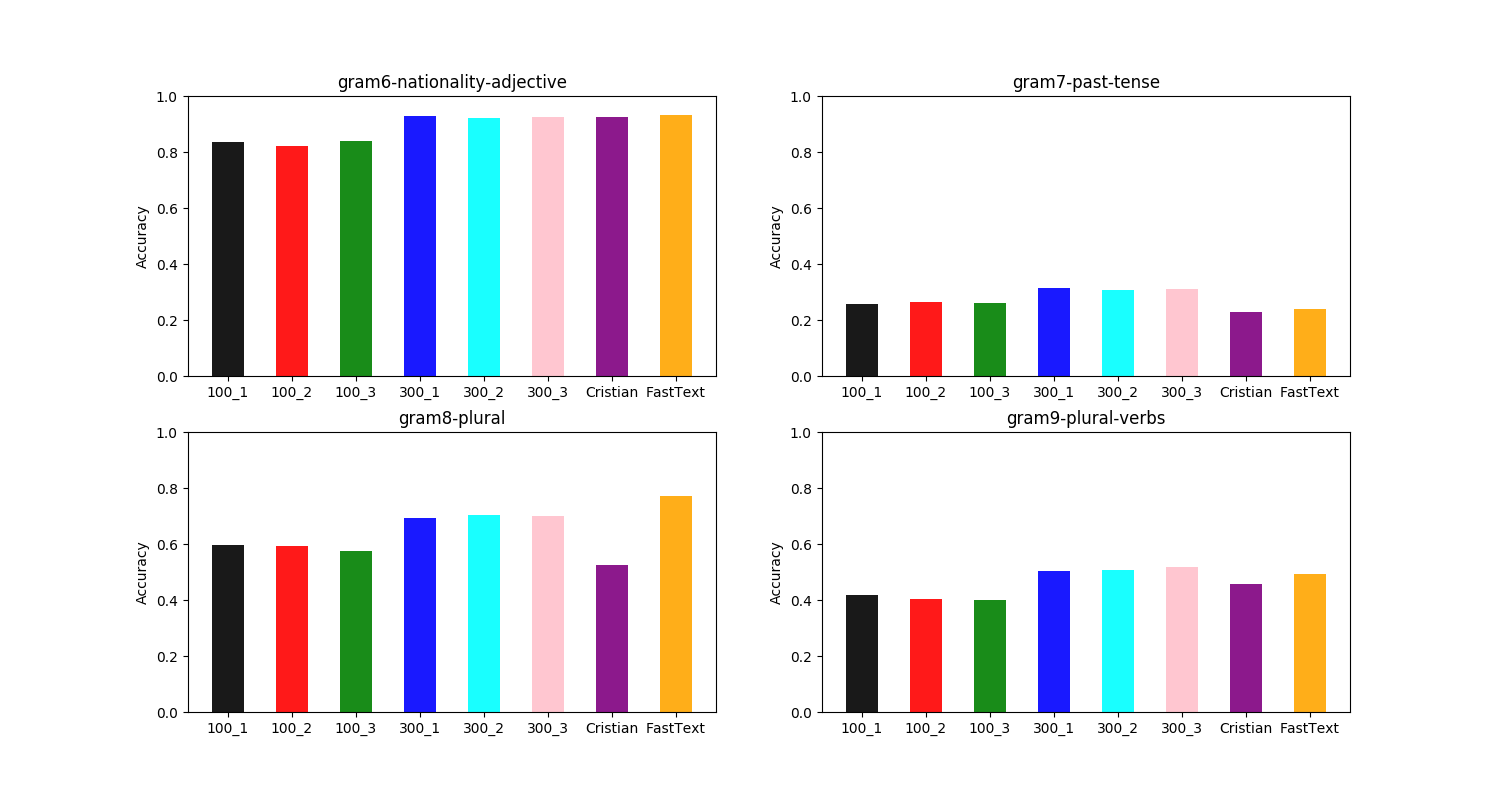
\includegraphics[width=1\textwidth]{plot3.png}
  \end{center}
\end{frame}

\begin{frame}{Modelo: Validación - Word2Vec accuracy}
  \begin{center}
    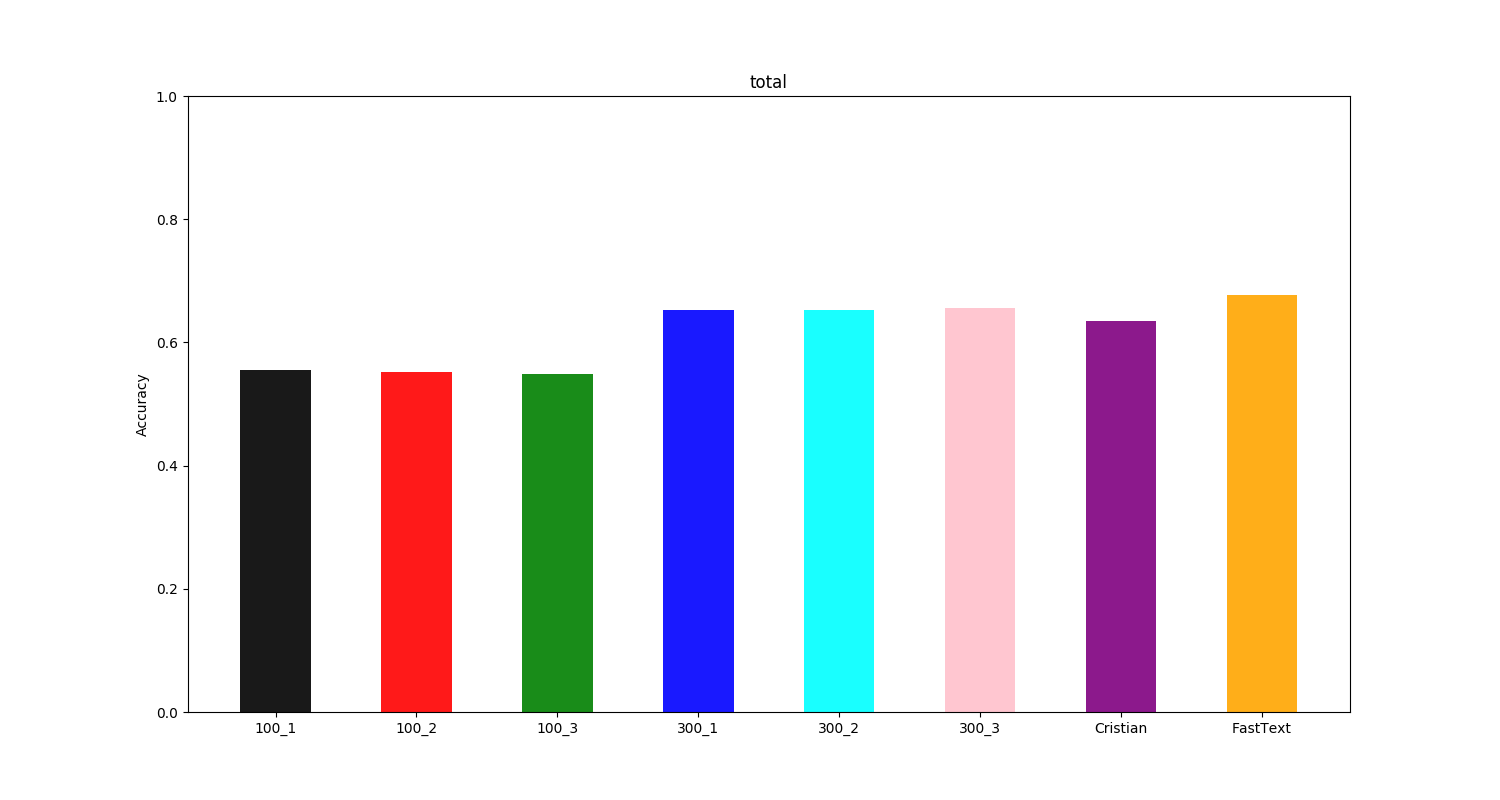
\includegraphics[width=1\textwidth]{total.png}
  \end{center}
\end{frame}

\begin{frame}{Modelo: Validación - Tagger}
  \begin{itemize}[<+->]
    \item Tagger implementado en práctico
    \item Agregamos la feature de palabras out-of-vocabulary
  \end{itemize}
\end{frame}


\begin{frame}{Modelo: Validación - Tagger}
  \begin{center}
    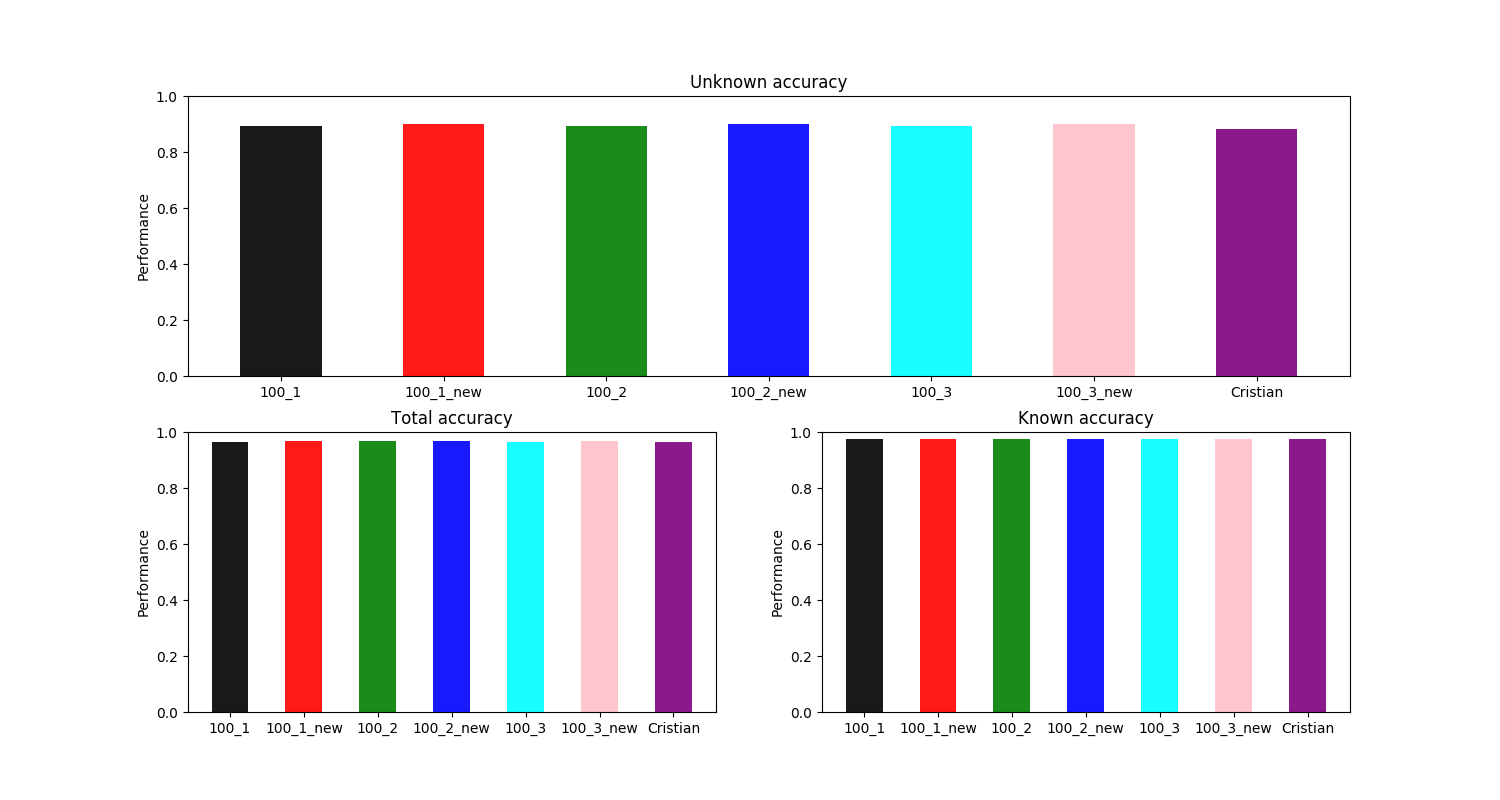
\includegraphics[width=1\textwidth]{tagger1.png}
  \end{center}
\end{frame}


\begin{frame}{Fin}
  \begin{center}
    Gracias! \\ Preguntas?
  \end{center}
\end{frame}


\begin{frame}{Referencias}
  \begin{itemize}
    \item https://github.com/juansca/WordVectors
    \item https://github.com/facebookresearch/fastText
    \item http://crscardellino.me/SBWCE/
    \item https://radimrehurek.com/gensim/models/word2vec.html
    \item https://www.quora.com/Is-it-compulsory-to-remove-stop-words-with-word2vec
    \item https://stackoverflow.com/questions/34721984/stopword-removing-when-using-the-word2vec

  \end{itemize}
\end{frame}


\defverbatim[colored]\lstI{
\begin{lstlisting}[language=Python]
  KNeighborsRegressor(n_neighbors, weights, algorithm,
                      leaf_size, p, metric,
                      metric_params, n_jobs, **kargs)
\end{lstlisting}
}

\appendix

\end{document}

%% \begin{frame}{Blocks}
%%   Three different block environments are pre-defined and may be styled with an
%%   optional background color.

%%   \begin{block}{Default}
%%     Block content.
%%   \end{block}

%%   \begin{alertblock}{Alert}
%%     Block content.
%%   \end{alertblock}

%%   \begin{exampleblock}{Example}
%%     Block content.
%%   \end{exampleblock}
%%   \stepcounter{beamerpauses}
%%   \begin{itemize}[<+->]
%%     \item Hola
%%     \item Chau
%%   \end{itemize}
%% \end{frame}
